\documentclass[aspectratio=169, 10pt]{beamer}

\usetheme{metropolis}
\usetikzlibrary{shapes, snakes}

\setbeamercolor{background canvas}{bg=white}

\metroset{
  numbering=fraction,
  progressbar=frametitle,
  block=fill,
}

\usefonttheme[onlymath]{serif}

\usepackage[ngerman]{babel}
\usepackage[style=iso-numeric]{biblatex}
\usepackage{csquotes}
\usepackage{mathtools, graphicx, booktabs, pgfplots}
\usepackage[font=footnotesize]{caption}
\usepackage{hyperref}

\addbibresource{bibliography.bib}
\graphicspath{{./Grafiken/}}
\captionsetup{belowskip=0pt}

\title{Algorithmik zur Optimierung in neuronalen Netzwerken}
\subtitle{Gradient Descent und Backpropagation}
\institute{Hochschule Esslingen --- University of Applied Sciences}
\author{Tim Hilt}
\date{Date: tbd}

\begin{document}

\begin{frame}
  \maketitle
\end{frame}

\begin{frame}{Gliederung}
  \tableofcontents
\end{frame}

\section{Supervised Learning}%
\label{sec:supervised}

\begin{frame}{Machine Learning Workflow}
  \begin{figure}[!htbp]
    \centering
    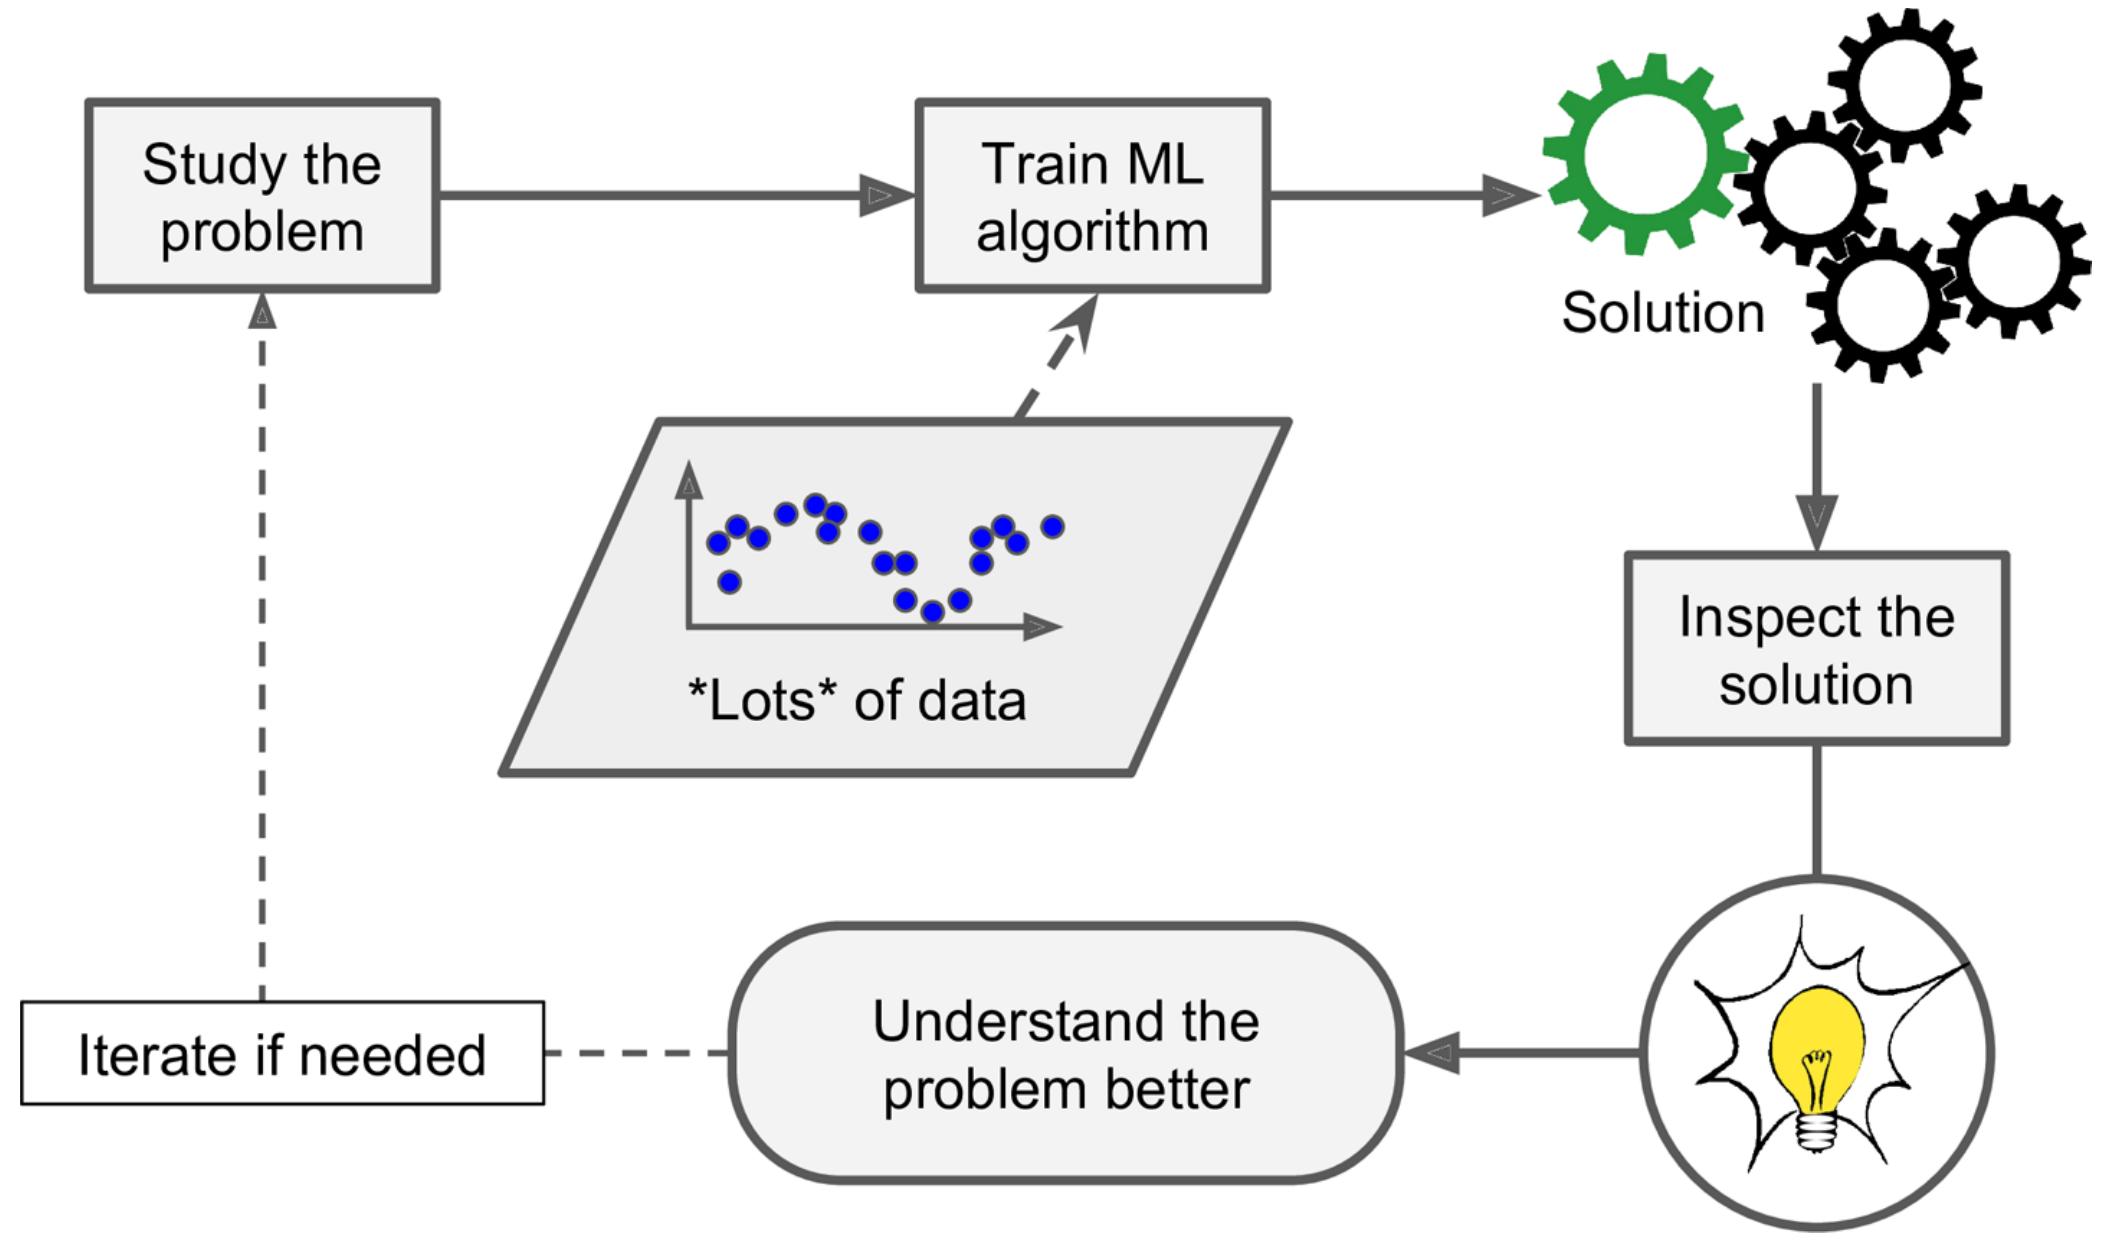
\includegraphics[width=10cm]{ml_workflow}
    \caption{Machine Learning Workflow \parencite{geron2019hands}}%
    \label{fig:workflow}
  \end{figure}
\end{frame}

\begin{frame}{Supervised Learning}
  \begin{figure}[!htbp]
    \centering
    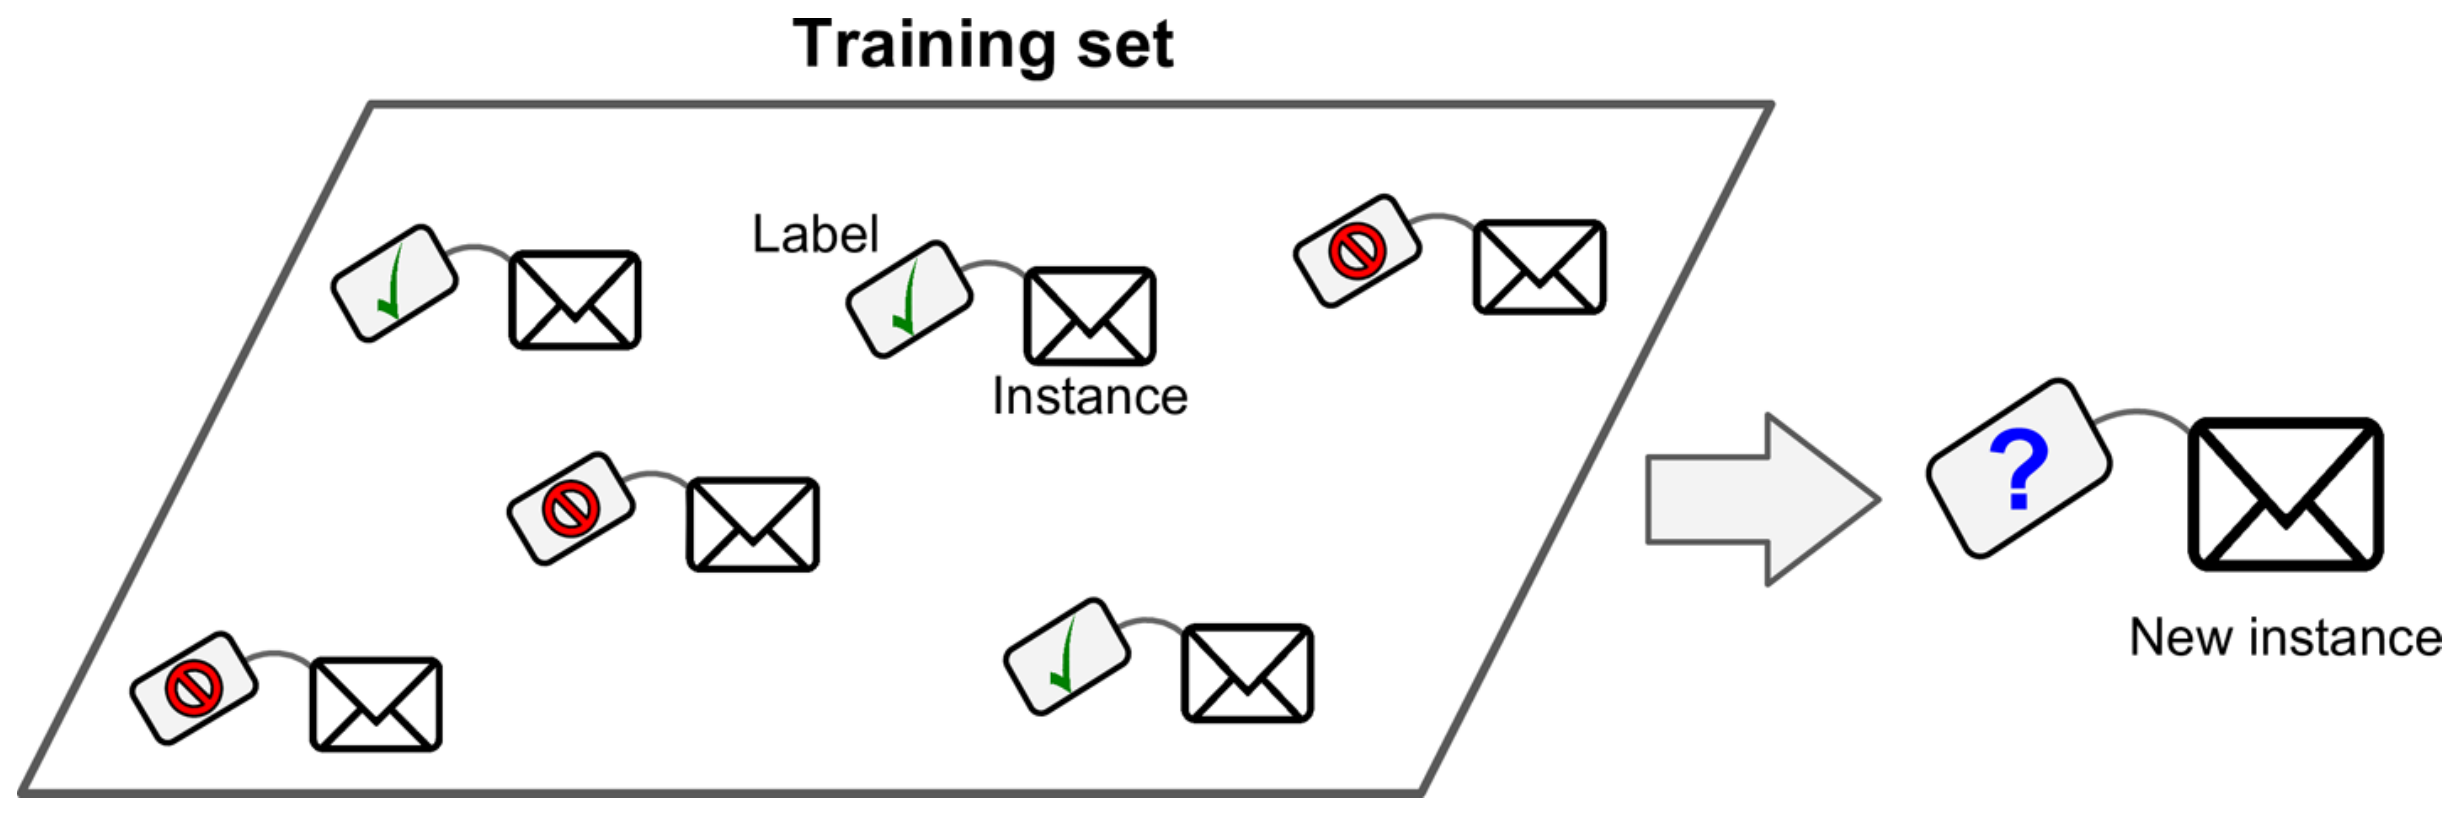
\includegraphics[width=8cm]{data}
    \caption{Struktur der Daten bei Supervised Learning \parencite{geron2019hands}}%
    \label{fig:data}
  \end{figure}

  \only<2->{
    \small
    \begin{block}{Definition Supervised Learning}
      \enquote{In supervised learning, the dataset is the collection of labeled examples
      \(\{(\mathbf{x}_i, y_i)\}_{i=1}^N\). Each element \(\mathbf{x}_i\) among
      \(N\) is called a feature vector. A feature vector is a vector in which each
      dimension \(j = 1, \ldots , D\) contains a value that describes the example
      somehow [\ldots]. The goal of a supervised learning algorithm is to use the
      dataset to produce a model, that takes a feature vector \(\mathbf{x}\) as
      input and outputs information that allow deducing the label \(\hat{y}\) for
      this feature vector.} \parencite{burkov2019hundred}
    \end{block}
  }
\end{frame}

\begin{frame}{Beispiel: Datensatz für Supervised Learning}
  \begin{minipage}{.6\textwidth}
    \centering
    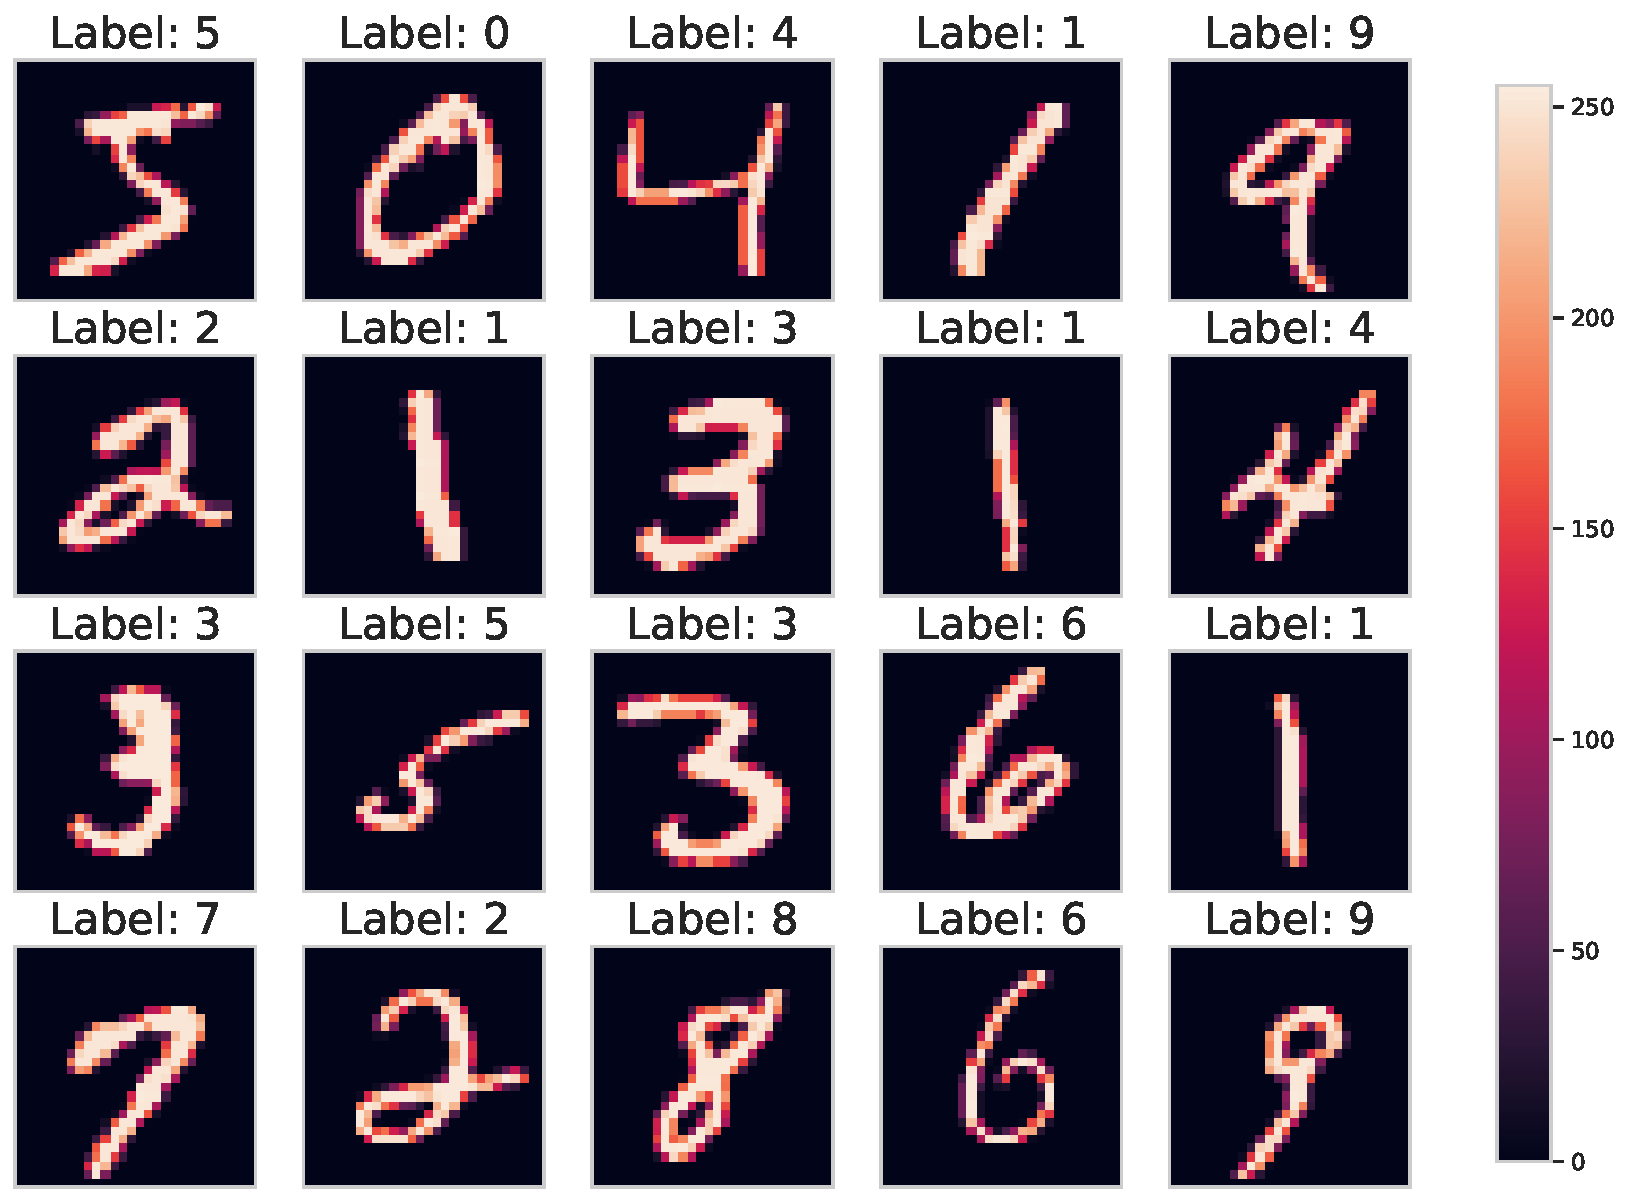
\includegraphics[width=\textwidth]{mnist}
  \end{minipage}\hfill%
  \begin{minipage}{.4\textwidth}
    \begin{itemize}
    \item Insgesamt 70000 Bilder
    \item Bildgröße: 28 \(\times\) 28 Pixel
    \item Abgebildet: Handgeschriebene Ziffern von 0 bis 9
    \item Quelle: Yann LeCun et al \parencite{lecun1998gradient}
    \end{itemize}
  \end{minipage}
\end{frame}

\begin{frame}{Beispiel: Datensatz für Supervised Learning}
  \begin{minipage}{.6\textwidth}
    \centering 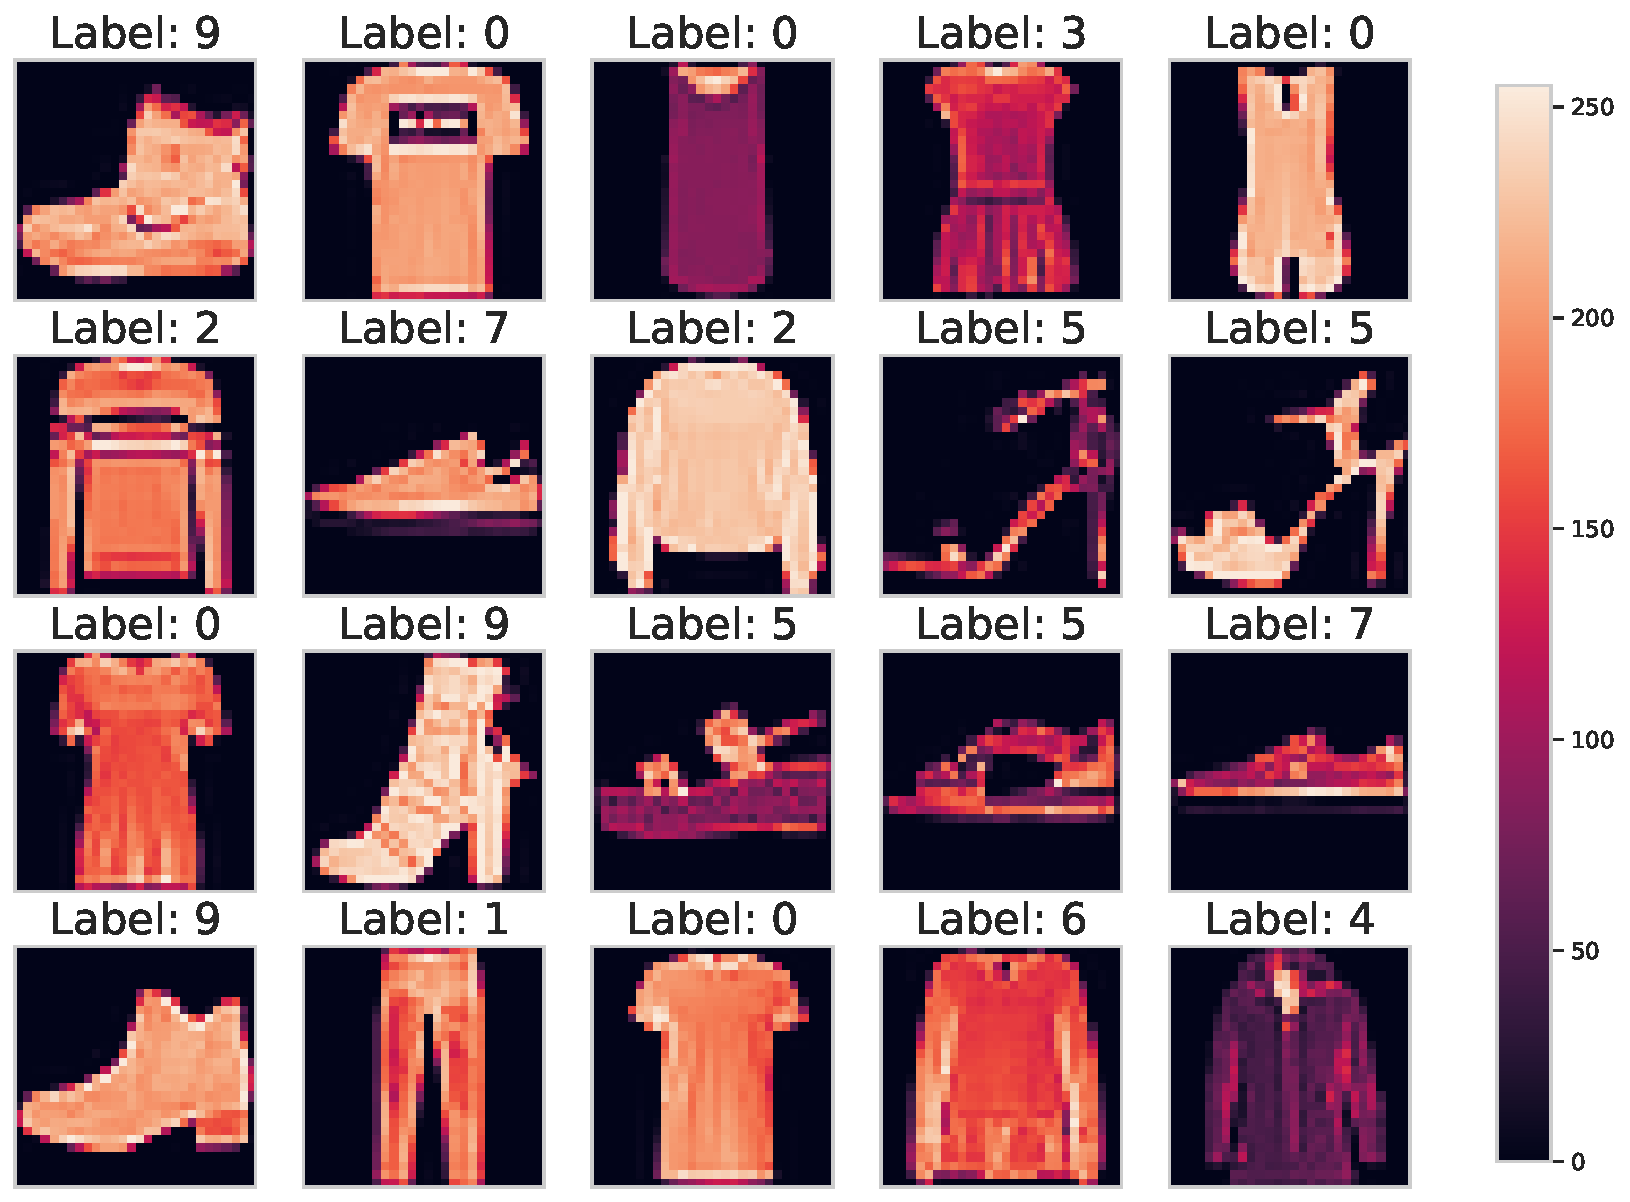
\includegraphics[width=\textwidth]{fashion_mnist}
  \end{minipage}\hfill%
  \begin{minipage}{.4\textwidth}
    \begin{itemize}
    \item Insgesamt 70000 Bilder
    \item Bildgröße: 28 \(\times\) 28 Pixel
    \item Abgebildet: Kleidungsstücke 
    \item Quelle: Zalando Research \parencite{xiao2017fashion}
    \end{itemize}

    \vspace{.5cm}

    \tiny

    \centering
    \begin{tabular}{ll}
      \toprule
      \textbf{Label} & 	\textbf{Description}\\
      \midrule
      0 & 	T-shirt/top\\
      1 & 	Trouser\\
      2 & 	Pullover\\
      3 & 	Dress\\
      4 & 	Coat\\
      5 & 	Sandal\\
      6 & 	Shirt\\
      7 & 	Sneaker\\
      8 & 	Bag\\
      9 & 	Ankle boot\\
      \bottomrule
    \end{tabular}

  \end{minipage}

\end{frame}

\section{Künstliche Neuronale Netze}%
\label{sec:ann}

\begin{frame}{Künstliches Neuron}
  \begin{minipage}{.65\textwidth}
    \begin{tikzpicture}[->, >=stealth, thick, scale=.8]
      \node [circle split,draw,rotate=90] (z) at (0, 0) {\rotatebox{-90}{$\displaystyle\sum$} \nodepart{lower} \rotatebox{-90}{$\sigma(z)$}};
      \foreach \i in {5,...,1} {
        \node (x-\i) at (-7, 4.5+1.5*-\i) {\(x_{\i}\)};
        \path (x-\i) edge node[above] {\(w_{\i}\)} (z);
      }
      \node (y) at (4, 0) {\(a\)};
      \path (z) edge (y);
      \node (b) at (0, 2.5) {\(b\)};
      \draw (b) -- (z);
    \end{tikzpicture}
  \end{minipage}%
  \begin{minipage}{.35\textwidth}
    \uncover<2->{
      \begin{flushright}
        \begin{tabular}{cl}
          \toprule
          \(\mathbf{x}\)  & Inputvektor\\
          \(\mathbf{w}\)  & Gewichtsvektor\\
          \(b\)  & Bias\\
          \(z\)  & Zwischensumme \(\left(\sum\right)\)\\
          \(\sigma(x)\)  & Aktivierungsfunktion\\
          \(a\)  & Aktivierung/ Output\\
          \bottomrule
        \end{tabular}
      \end{flushright}
    }
  \end{minipage}

  \only<3>{
    \[z = \sum_ix_iw_i + b = \mathbf{xw} + b\]

    {\centering\(\Rightarrow z\) wird für spätere Parameteroptimierung benötigt\par}
  }
\end{frame}

\begin{frame}{Aktivierungsfunktion \(\sigma(x)\)}
  \begin{minipage}{.45\textwidth}
    \(\Rightarrow\) Es gibt eine Vielzahl verschiedener Aktivierungsfunktionen für unterschiedliche Problemstellungen, für uns soll jedoch lediglich die \textbf{Sigmoid-Funktion} relevant sein:

    \vspace{1cm}

    \[\sigma(x) = \frac{1}{1 + e^{-x}}\]
  \end{minipage}\hfill%
  \begin{minipage}{.5\textwidth}
    \only<2>{
      \begin{tikzpicture}
        \begin{axis}[width=\textwidth, mlineplot, samples=50, ymin=-.1, ymax=1.1, domain=-10:10, title=Sigmoid-Funktion, xlabel=\(x\), ylabel=\(\sigma(x)\)]
          \addplot{1/(1+exp(-x))};
        \end{axis}
      \end{tikzpicture}
    }
  \end{minipage}

\end{frame}

\begin{frame}{Architektur eines neuronalen Netzes}
  \def\layersep{2.5cm}
  \begin{center}
    \begin{tikzpicture}[->, >=stealth]
      \tikzstyle{every pin edge}=[<-,shorten <=1pt]
      \tikzstyle{neuron}=[circle,draw,minimum size=17pt,inner sep=0pt]
      
      % Draw the input layer nodes
      \foreach \y in {1,...,5}
      \node[neuron, pin=left:] (I-\y) at (0,-\y) {};

      % Draw the nodes for the second hidden layer
      \foreach \y in {1,...,7}
      \path[yshift=(7cm - 5cm)/2] node[neuron] (H1-\y) at (\layersep,-\y cm) {};

      % Draw the nodes for the second hidden layer
      \foreach \y in {1,...,5}
      \path node[neuron] (H2-\y) at (2*\layersep,-\y cm) {};

      % Draw the output layer nodes
      \foreach \y in {1,...,3}
      \path[yshift=(3cm - 5cm)/2] node[neuron,pin={[pin edge={->}]right:}] (O-\y) at (3*\layersep,-\y cm) {};

      \foreach \source in {1,...,5}
      \foreach \dest in {1,...,7}
      \path (I-\source) edge (H1-\dest);

      \foreach \source in {1,...,7}
      \foreach \dest in {1,...,5}
      \path (H1-\source) edge (H2-\dest);

      \foreach \source in {1,...,5}
      \foreach \dest in {1,...,3}
      \path (H2-\source) edge (O-\dest);
    \end{tikzpicture}
  \end{center}

\end{frame}

\section{Training}
\label{sec:train}

\subsection{Loss-Funktion}
\label{sec:loss}



\subsection{Gradient Descent}
\label{sec:graddesc}



\subsection{Backpropagation}
\label{sec:backprop}

\begin{frame}{Backpropagation}
  Es werden vier Gleichungen benötigt:

  Error im Output-Layer:

  Error einzelner Neuronen:

  \[\delta_j^L = \frac{\partial C}{\partial a_j^L} \sigma' \left(z_j^L\right)\]

  Vektorisiert:

  \[\delta^L = \nabla_aC \odot \sigma'(z^L)\]

  Aufgelöst, wenn MSE benutzt:

  \[\delta^L = (a^L - y) \odot \sigma'(z^L)\]
\end{frame}

\begin{frame}{Backpropagation}
  Error im Layer \(l\) hinsichtlich Error im nächsten Layer \(\delta^{l+1}\)

  \[\delta^l = \left(\left(w^{l+1}\right)^T\delta^{l+1}\right) \odot
    \sigma'\left(z^l\right)\]

  \begin{itemize}
  \item Rekursive Definition durch Verwendung von \(\delta^l\) in Abhängigkeit
    von \(\delta^{l+1}\)
  \item Wenn anfangs \(\delta^L\) in die Gleichung gegeben wird kann der Error
    rekursiv für jeden vorhergehenden Layer berechnet werden
  \end{itemize}
\end{frame}

\begin{frame}{Backpropagation}
  \begin{align*}
    \delta^L &= \nabla_aC \odot \sigma' \left(z^L\right)\\[1em]
    \delta^l &= \left(\left(w^{l+1}\right)^T \delta^{l+1}\right) \odot
               \sigma'\left(z^l\right)\\[1em]
    \frac{\partial C}{\partial b^l_j} &= \delta^l_j\\[1em]
    \frac{\partial C}{\partial w^l_{jk}} &= a^{l-1}_k\delta^l_j
  \end{align*}
\end{frame}

\begin{frame}{Beispiel}
  Pass
\end{frame}

\begin{frame}[standout]
  Fragen?
\end{frame}

\printbibliography[title=Literaturverzeichnis]

\end{document}